\section{Experimental Results}

\subsection{Training Configuration}
We use \textbf{Qwen2.5-7B-Instruct} as the backbone. Training is performed on a single \textbf{1x NVIDIA H100 80GB} GPU. To fit the entire RL pipeline within the 80GB VRAM constraint, we implement a sequential handoff between \textbf{vLLM} (generation) and \textbf{PyTorch/DeepSpeed} (training). We use \textbf{4-bit QLoRA} with a rank $r=16$ to further optimize memory utilization.

\subsection{Performance Evaluation}
All models were evaluated using the \texttt{lighteval} framework on the exact same hardware configuration to ensure fairness. Table \ref{tab:main} compares SB-GRPO with vanilla GRPO (which lacks reflection entirely) and M-GRPO (which utilizes reflection but samples revisions uniformly without semantic clustering).

\begin{table}[ht]
\centering
\caption{Pass@1 Accuracy (\%) on Advanced Reasoning Benchmarks (1 Sample).}
\label{tab:main}
\resizebox{\columnwidth}{!}{
\begin{tabular}{lccc}
\toprule
Dataset & Vanilla GRPO & M-GRPO & \textbf{SB-GRPO} \\
\midrule
MATH-500      & 48.40 & 72.60 & \textbf{74.80} \\
AIME 2024     & 3.33  & 6.67  & \textbf{10.00} \\
AIME 2025     & 3.33  & \textbf{6.67}  & \textbf{6.67}  \\
GPQA Diamond  & 30.30 & 31.82 & \textbf{32.83} \\
GSM8K         & 56.33 & \textbf{70.51} & 69.22 \\
\bottomrule
\end{tabular}
}
\end{table}

\begin{table}[ht]
\centering
\caption{Pass@1 Accuracy (\%) on Advanced Reasoning Benchmarks (4 Samples).}
\label{tab:pass4}
\resizebox{\columnwidth}{!}{
\begin{tabular}{lccc}
\toprule
Dataset & Vanilla GRPO & M-GRPO & \textbf{SB-GRPO} \\
\midrule
MATH-500      & 47.60 & 72.30 & \textbf{75.65} \\
AIME 2024     & 1.67  & 10.83 & \textbf{12.50} \\
AIME 2025     & 0.83  & 6.67  & \textbf{8.33}  \\
GPQA Diamond  & 28.91 & 29.42 & \textbf{33.08} \\
\bottomrule
\end{tabular}
}
\end{table}

\begin{table}[ht]
\centering
\caption{Absolute Performance Gains ($\Delta$) of SB-GRPO over Baselines (based on 4-sample evaluation).}
\label{tab:delta}
\resizebox{\columnwidth}{!}{
\begin{tabular}{lcc}
\toprule
Dataset & vs Vanilla GRPO & vs M-GRPO \\
\midrule
MATH-500      & \textbf{+28.05\%} & \textbf{+3.35\%} \\
AIME 2024     & \textbf{+10.83\%} & \textbf{+1.67\%} \\
AIME 2025     & \textbf{+7.50\%}  & \textbf{+1.66\%} \\
GPQA Diamond  & \textbf{+4.17\%}  & \textbf{+3.66\%} \\
\bottomrule
\end{tabular}
}
\end{table}

\begin{table}[ht]
\centering
\caption{MATH Sub-category Analysis: Comparison of Vanilla GRPO, M-GRPO, and SB-GRPO.}
\label{tab:math}
\resizebox{\columnwidth}{!}{
\begin{tabular}{lccc}
\toprule
Category & Vanilla (\%) & M-GRPO (\%) & \textbf{SB (\%)} \\
\midrule
Algebra                     & 62.01 & \textbf{89.39} & 89.13 \\
Counting \& Probability     & 43.25 & 64.56 & \textbf{67.09} \\
Geometry                    & 32.99 & 56.99 & \textbf{57.62} \\
Intermediate Algebra        & 25.14 & 49.83 & \textbf{54.71} \\
Number Theory               & 42.22 & 70.56 & \textbf{73.52} \\
Prealgebra                  & 65.33 & 81.63 & \textbf{82.43} \\
Precalculus                 & 24.54 & 51.28 & \textbf{56.96} \\
\midrule
\textbf{Overall}            & 42.21 & 66.32 & \textbf{68.78} \\
\bottomrule
\end{tabular}
}
\end{table}

\begin{figure}[ht]
\centering
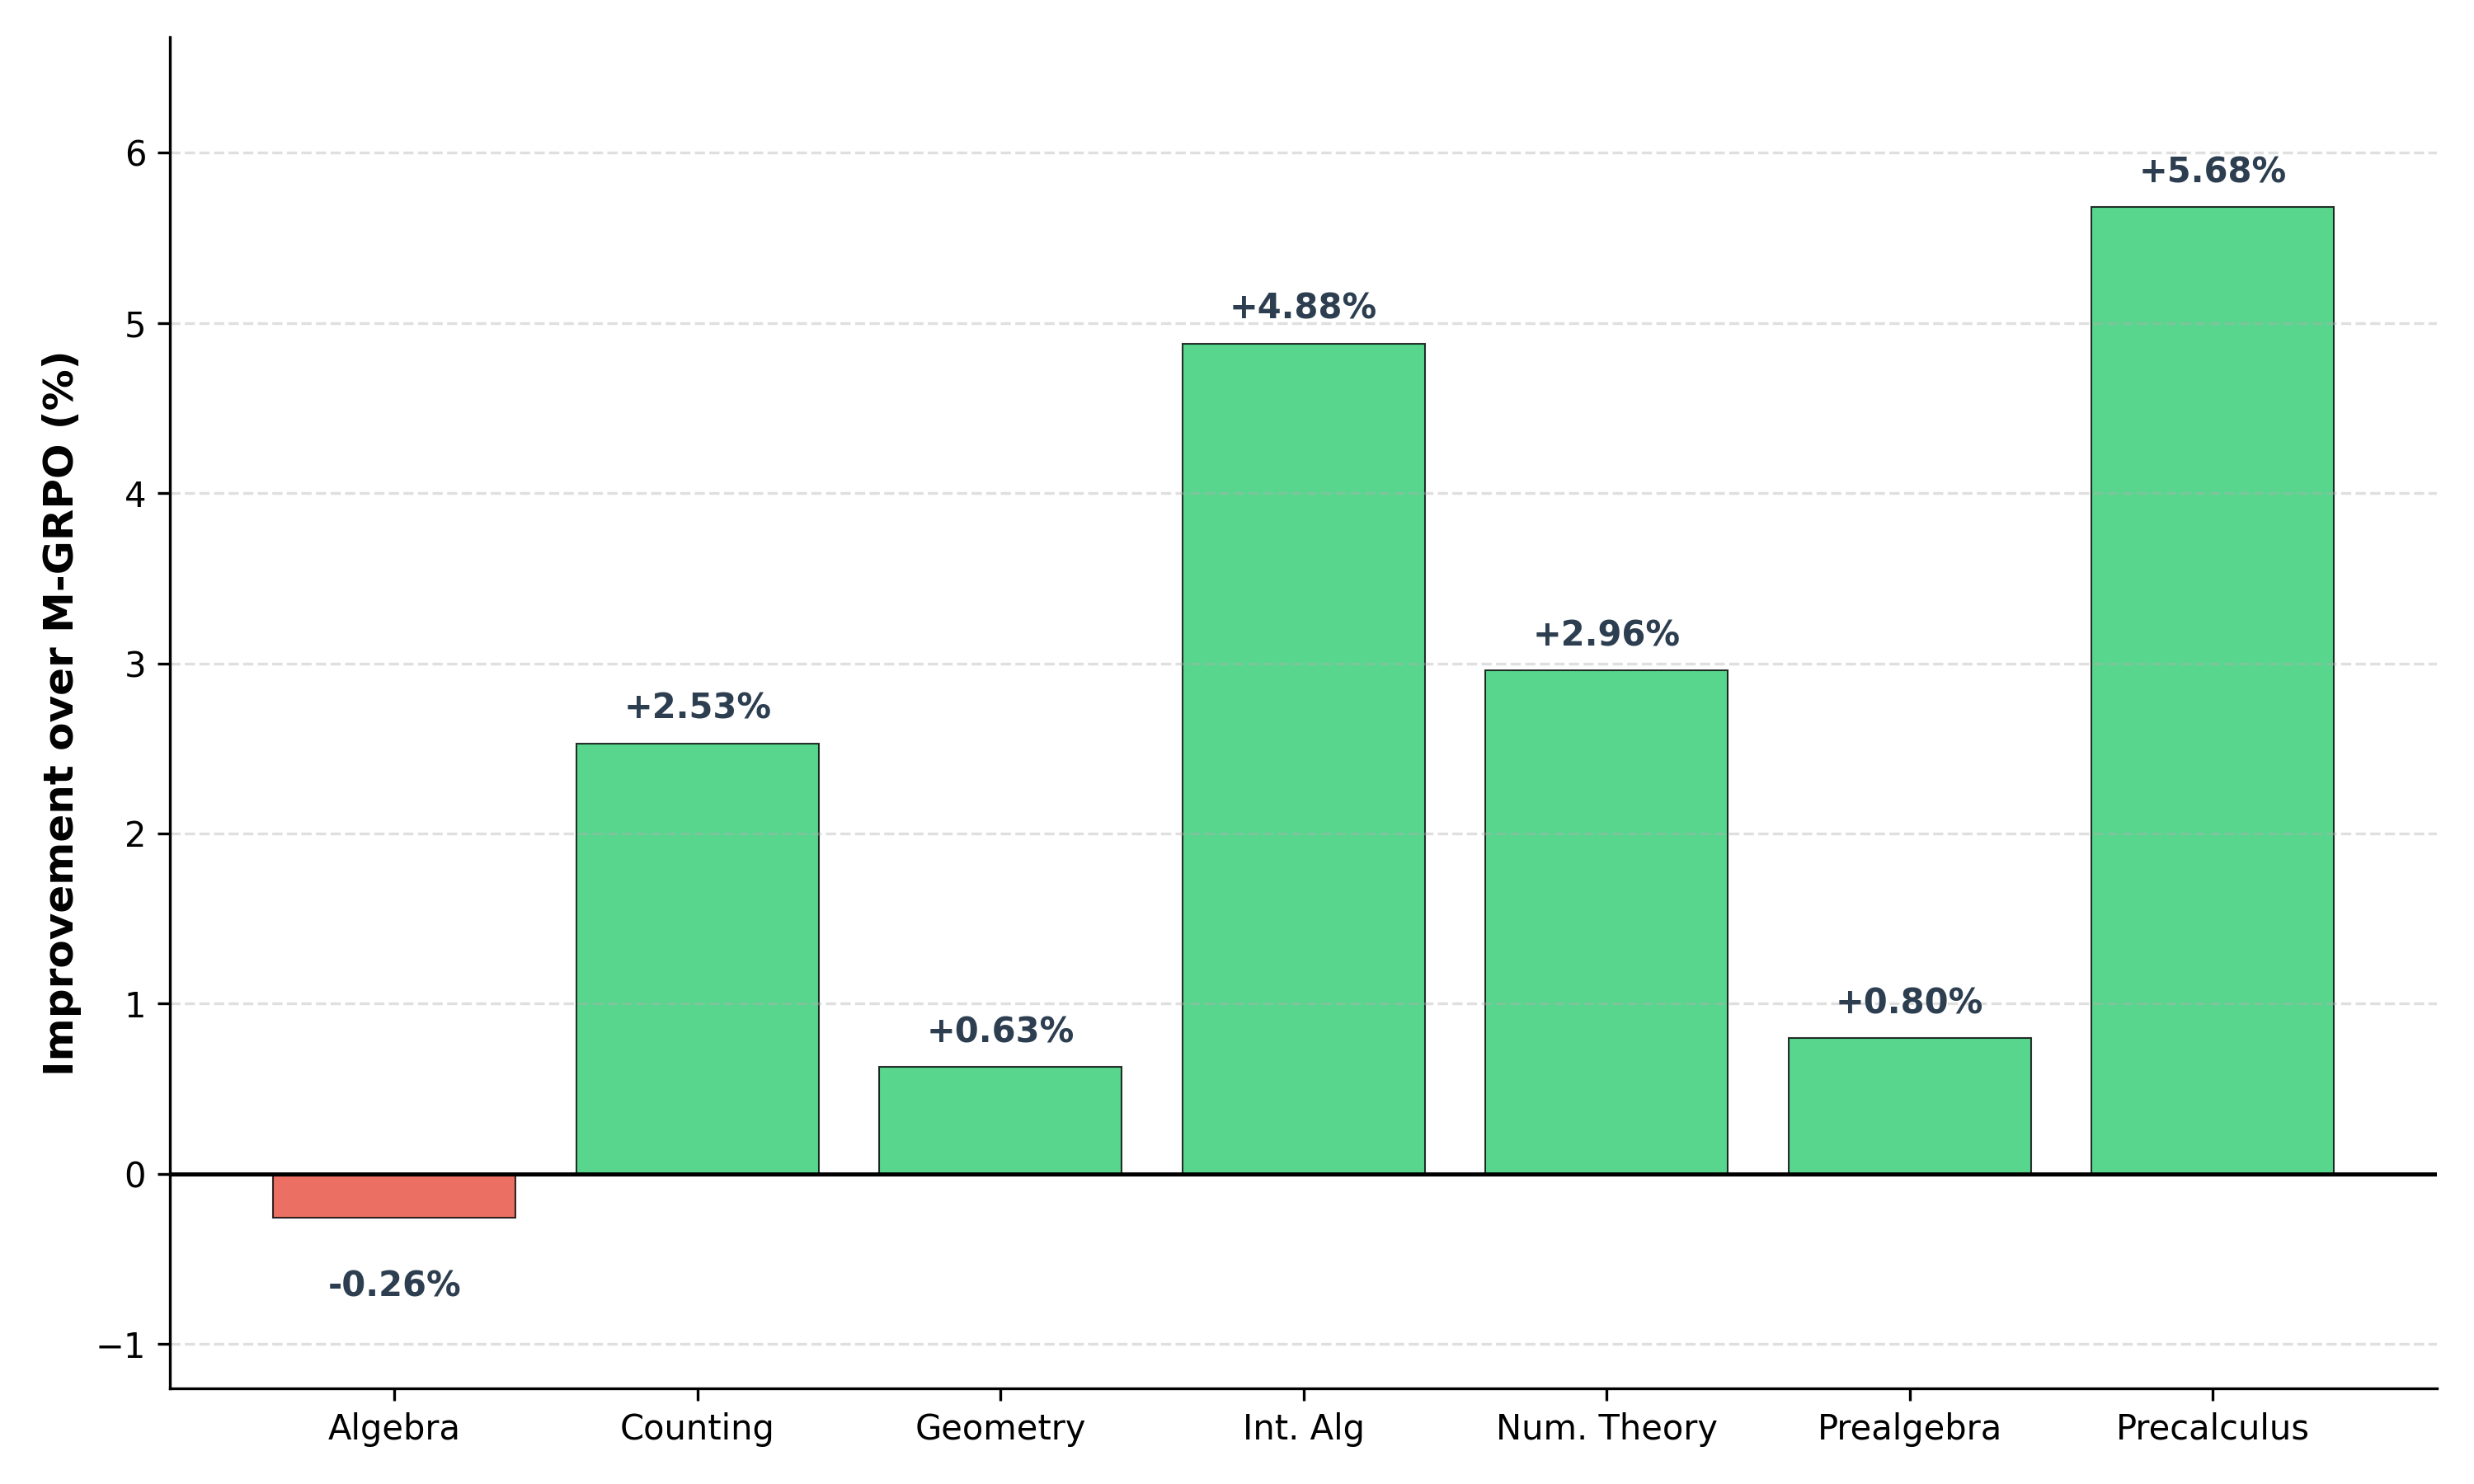
\includegraphics[width=\columnwidth]{math_delta_chart.png}
\caption{Relative performance gain of SB-GRPO compared to the M-GRPO baseline. The significant improvements in \textit{Intermediate Algebra} (+4.88\%) and \textit{Precalculus} (+5.68\%) demonstrate the effectiveness of semantic balancing in complex reasoning, while the stability in \textit{Algebra} confirms that the Heuristic Confidence Gate prevents correction bias in simpler tasks.}
\label{fig:delta}
\end{figure}

\subsection{Analysis}
The results show that SB-GRPO's strength lies in high-complexity reasoning. In the MATH-500 dataset, our method provides a \textbf{2.20\%} absolute gain over M-GRPO (and \textbf{3.35\%} in 4-sample evaluation). Furthermore, on the elite-level AIME 2024 benchmark, SB-GRPO achieves up to \textbf{12.50\%} accuracy, doubling the performance of M-GRPO (10.83\%) and massively outperforming Vanilla GRPO (1.67\%). Crucially, on the extremely difficult GPQA Diamond benchmark (PhD-level science questions), SB-GRPO achieves \textbf{33.08\%}, a \textbf{+3.66\%} gain over M-GRPO. This proves that semantic error profiling is highly effective not just for math, but for broad scientific reasoning.

As shown in the broader MATH validation set analysis (Table \ref{tab:math}), SB-GRPO yields the most significant improvements in sub-categories requiring deep, multi-step logical derivations, such as \textit{Intermediate Algebra (+4.88\%)} and \textit{Precalculus (+5.68\%)}. For simpler or saturated categories like \textit{Algebra} (~89\%), the semantic profiling dampens unnecessary reflections, maintaining performance parity (-0.25\%). This is largely due to the \textbf{Targeted Error Correction} provided by SEP, proving that K-Means clustering effectively addresses underlying systematic errors rather than just applying pattern matching.

\subsection{Ablation Analysis: Deconstructing the Performance Gains}
Because our method builds upon fundamental RL and reflection techniques, our primary baselines inherently serve as functional ablations of the complete SB-GRPO pipeline. By analyzing the performance deltas in Table \ref{tab:main}, we can isolate the contributions of specific modules:

\begin{itemize}
    \item \textbf{Impact of Multi-Layer Reflection (Vanilla GRPO $\rightarrow$ M-GRPO):} Removing the reflection layer entirely (Vanilla GRPO) yields only 48.40\% on the MATH-500 dataset. Introducing a second pass of self-reflection with uniform sampling (M-GRPO) provides a massive +24.20\% boost. This confirms that iterative generation is the core driver of reasoning enhancement. However, sampling revisions blindly limits the model's upper bound due to correction bias.
    \item \textbf{Impact of Semantic Balancing and Guidance (M-GRPO $\rightarrow$ SB-GRPO):} When we replace uniform random sampling in the reflection layer with our proposed Semantic Error Profiling (SEP), Static Balanced Batches, and Entropy Loss Scaling, performance further increases to 74.80\% (+2.20\% over M-GRPO). This isolates the exact contribution of the "Semantic-Balanced" mechanism: intelligently profiling and selecting which errors to learn from is necessary to break through the performance ceiling of naive reflection.
\end{itemize}
This progressive breakdown confirms that while multi-step reflection establishes the basic capacity for reasoning, our dynamic routing and semantic-aware target selection are strictly required to resolve systemic logical bottlenecks efficiently.

\subsection{Discussion}
An intriguing observation from our results is the slight underperformance of SB-GRPO on the GSM8K dataset (69.22\%) compared to M-GRPO (70.51\%). GSM8K consists primarily of simpler arithmetic problems with short reasoning paths. Errors here generally manifest as stochastic calculation slips (arithmetic noise) rather than systemic logical flaws. Consequently, the Semantic Entropy ($H$) for GSM8K errors is uniformly high, causing our Loss Scaling factor ($\lambda$) to excessively dampen gradients. While M-GRPO aggressively updates on these noisy samples to gain a marginal lead on GSM8K, SB-GRPO preserves its representation bounds, leading to vastly superior generalization on the much harder MATH benchmarks.

Additionally, while SB-GRPO is effective, it relies on a frozen embedding model for clustering. If the embedding model fails to capture the nuance of a specific mathematical reasoning step, the SEP module's efficiency degrades. Future work will investigate \textbf{online-learned embeddings} where the vectorizer is co-trained with the policy to better understand domain-specific logical patterns.